%% Hlavička %%
\newcommand{\cvut}{ČESKÉ VYSOKÉ UČENÍ TECHNICKÉ
V~PRAZE}
\newcommand{\cvuten}{CZECH TECHNICAL UNIVERSITY \newline IN
PRAGUE}
\newcommand{\fjfi}{Fakulta jaderná a fyzikálně inženýrská}
\newcommand{\fjfien}{Faculty of Nuclear Sciences and Physical
Engineering}
\newcommand{\kf}{Katedra Fyziky} 
\newcommand{\kfen}{Department of Physics}
\newcommand{\program}{Aplikace přírodních věd} 
\newcommand{\obor}{Jaderná a částicová fyzika} 

\newcommand{\druh}{Bakalářská práce} % nebo "Diplomová práce"
\newcommand{\druhen}{Bachelor thesis} % nebo "Diplomová práce"
\newcommand{\woman}{} 

\newcommand{\logoCVUT}{
\includegraphics{figures/symbol_cvut_konturova_verze_cb.pdf}}

% přesně podle formuláře "Zadání bak./dipl. práce" VYPLŇTE:
\newcommand{\nazevcz}{Procesy s výměnou pomeronu na experimentu STAR}    % český název práce (přesně podle zadání!)
\newcommand{\nazeven}{Pomeron exchange processes at the STAR experiment}          % anglický název práce (přesně podle zadání!)
\newcommand{\autor}{Michal Vranovský}   % vyplňte své jméno a příjmení (s akademickým titulem, máte-li jej)
\newcommand{\vedouci}{doc. Mgr. Jaroslav Bielčík, Ph.D.} % vyplňte jméno a příjmení vedoucího práce, včetně titulů, např.: do~c. Ing. Ivo Malý, Ph.D.
\newcommand{\pracovisteVed}{\kf, \fjfi, České vysoké učení technické v Praze} % ZMĚŇTE, pokud vedoucí Vaší práce není z KSI
\newcommand{\konzultant}{Ing. Tomáš Truhlář} % POKUD MÁTE určeného konzultanta, NAPIŠTE jeho jméno a příjmení
\newcommand{\pracovisteKonz}{\kf, \fjfi, České vysoké učení technické v Praze} % POKUD MÁTE konzultanta, NAPIŠTE jeho pracoviště

% podle skutečnosti VYPLŇTE:
\newcommand{\rok}{2023}  % rok odevzdání práce (jen rok odevzdání, nikoli celý akademický rok!)
\newcommand{\kde}{Praze} % studenti z Děčína ZMĚNÍ na: "Děčíně" (doplní se k "prohlášení")

\newcommand{\klicova}{Pomeron, Glueball, RHIC, STAR}   % zde NAPIŠTE česky max. 5 klíčových slov
\newcommand{\keyword}{Pomeron, Glueball, RHIC, STAR}       % zde NAPIŠTE anglicky max. 5 klíčových slov (přeložte z češtiny)
\newcommand{\abstrCZ}{Tématem této práce je studium procesů s výměnou \Pom omeronu, zvláště pak Dvojitá \Pom omeronová výměna. Úspěšný popis tohoto procesu by mohl znamenat krok k porozumění vázaných gluonových stavů, takzvaných glueballs. Data k analýze pocházejí z proton-protonových srážek při energii $\sqrt{s} = 510$ GeV naměřené na experimentu STAR, který se nachází na RHIC urychlovači v Brookhavenské národní laboratoři. Práce se zaměřuje na rekonstrukci neutrálních částic $K^0_S$ and $\Lambda^0$, které jsou vytvořeny v procesu $p+p \longrightarrow p+ K^0_S +p$ a $p + p \longrightarrow p + \Lambda^0 + p$. Tyto částice se rozpadají na páry $\pi^+ \pi^-$ a $p \pi^-$. Velmi důležité pro tuto analýzu je systém detektorů Římskych nádob, které jsou schopny rekonstruovat dráhy dopředně rozptýlených protonů, díky čemu jsme schopni měřit exkluzivní procesy.}  % zde NAPIŠTE abstrakt v češtině (cca 7 vět, min. 80 slov)

\newcommand{\abstrEN}{The topic of this thesis is the study \Pom omeron exchange processes, especially the Double \Pom omeron Exchange. A successful description of this process could mean a step towards the understanding of bound gluon states, glueballs. The analyzed data come from proton-proton collisions at $\sqrt{s} = 510$ GeV at the experiment STAR placed at the Relativistic Heavy Ion Collider located in Brookhaven National Laboratory. The focus is on the reconstruction of neutral particles, primarily $K^0_S$ and $\Lambda^0$, involved in process $p+p \longrightarrow p+ K^0_S +p$ and $p+p \longrightarrow p+ \Lambda^0 +p$. These  particles decay to pairs $\pi^+ \pi^-$ and $p \pi^-$ respectively. Key for this analysis is the Roman Pot system of detectors, which are able to reconstruct the tracks of forward scattered protons and therefore allow for study of exclusive processes. }
%\newcommand{\prohlaseni}{ Prehlasujem, že som svoju bakalársku prácu vypracoval\woman{} samostatne a použil\woman{} iba podklady (literatúru, projekty, SW atď.) uvedenú v priloženom zozname. \\ \\ Nemám závažný dôvod proti použitiu tohto školského diela v zmysle § 60 Zákona č.
%121/2000 Sb., o~autorskom práve, o právach súviciacich s~právom autorským a o~zmene niektorých zákonov(autorský zákon).}
\newcommand{\prohlaseni}{ Prohlašuji, že jsem svou bakalárskou práci vypracoval\woman{} samostatně a použil\woman{} jsem pouze podklady (literaturu, projekty, SW atd.) uvedenou v~přiloženém seznamu. \\ \\ Nemám závažný důvod proti užití tohoto školního díla ve~smyslu § 60 Zákona č.
121/2000 Sb., o~právu autorském, o~právech souvisejících s~právem autorským a
o~změně některých zákonů (autorský zákon).} 

\newcommand{\podekovani}{I would like to thank my supervisor \vedouci  ~for his guidance, his patience and valuable advice. I would also like to thank my consultant \konzultant ~for his constructive comments, help with analysis and guidance. At last, I would like to express my gratitude to my family and friends, who supported me throughout this journey.}


\thispagestyle{empty}

\begin{center}
    {\LARGE
        \cvuten\par
        \fjfien\par
        \kfen
    }
    \vspace{10mm}

   \vspace{10mm} \logoCVUT \vspace{15mm} 

   {\Large \tb{\druhen}}
   \vspace{15mm}

   {\huge \tb{\nazeven}\par}
  
   \vfill
   {\large
    \begin{tabular}{ll}
    Author: & \autor\\
    Supervisor: & \vedouci\\
    Consultant: & \konzultant \\
    Year: & \rok
    \end{tabular}
   }
\end{center}

\clearpage{\pagestyle{empty}\cleardoublepage} % prázdná stránka za~tou "titulní", bez čísla

%%%%%%%%%%%% TITULNÍ STRANA CZ %%%%%%%%%%%%
\newpage 
\thispagestyle{empty}

\begin{center}
    {\LARGE
        \cvut\par
        \fjfi
    }
    \vspace{10mm}

    \begin{tabular}{c}
        \tb{\kf} \\[3pt]   
        %\tb{Studijní program: \obor}\\
    \end{tabular}

   \vspace{10mm} \logoCVUT \vspace{15mm} 

   {\huge \tb{\nazevcz}\par}
   
   \vspace{15mm}
   {\Large \MakeUppercase{\druh}}

   \vfill
   {\large
    \begin{tabular}{ll}
    Vypracoval: & \autor\\
    Vedouci práce: & \vedouci\\
    Konzultant: & \konzultant \\
    Rok: & \rok
    \end{tabular}
   }
\end{center}
\clearpage{\pagestyle{empty}\cleardoublepage} % prázdná stránka za~tou "titulní", bez čísla

%%%%%%%%%%%% ZADÁNÍ PRÁCE %%%%%%%%%%%%

\newpage  
\thispagestyle{empty} 

% --- varianta A: zadání naskenované jako 2stránkové PDF:
\includepdf[pages={1,2}]{figures/zadani.pdf} % NAHRAĎTE správným souborem!
%
%% --- varianta B: zadání naskenované jako jednotlivé stránky:
%\includepdf[pages={1}]{zadani.pdf} % 1. strana zadání v PDF
%\newpage 
%\thispagestyle{empty} 
%\%

%\includepdf[pages={2}]{zadani.pdf} % 1. strana zadání v PDF
%\newpage 
%\thispagestyle{empty} 
%\

%\includepdf[pages={1}]{zadani2.pdf} % 2. strana zadání v PDF
%
%% --- varianta C: zadání naskenované jako 2 samostatné obrázky:
%% 1. strana zadání
%\begin{center}
%     \includegraphics[width=1\textwidth]{zadani1.jpg}
%\end{center}
%% 2. strana zadání
%\newpage  % SEM NESAHEJTE!
%\thispagestyle{empty} % SEM NESAHEJTE!
%\begin{center}
%     \includegraphics[width=1\textwidth]{zadani2.jpg}
%\end{center}


%%%%%%%%%%%% Prohlášení  %%%%%%%%%%%%
\newpage 


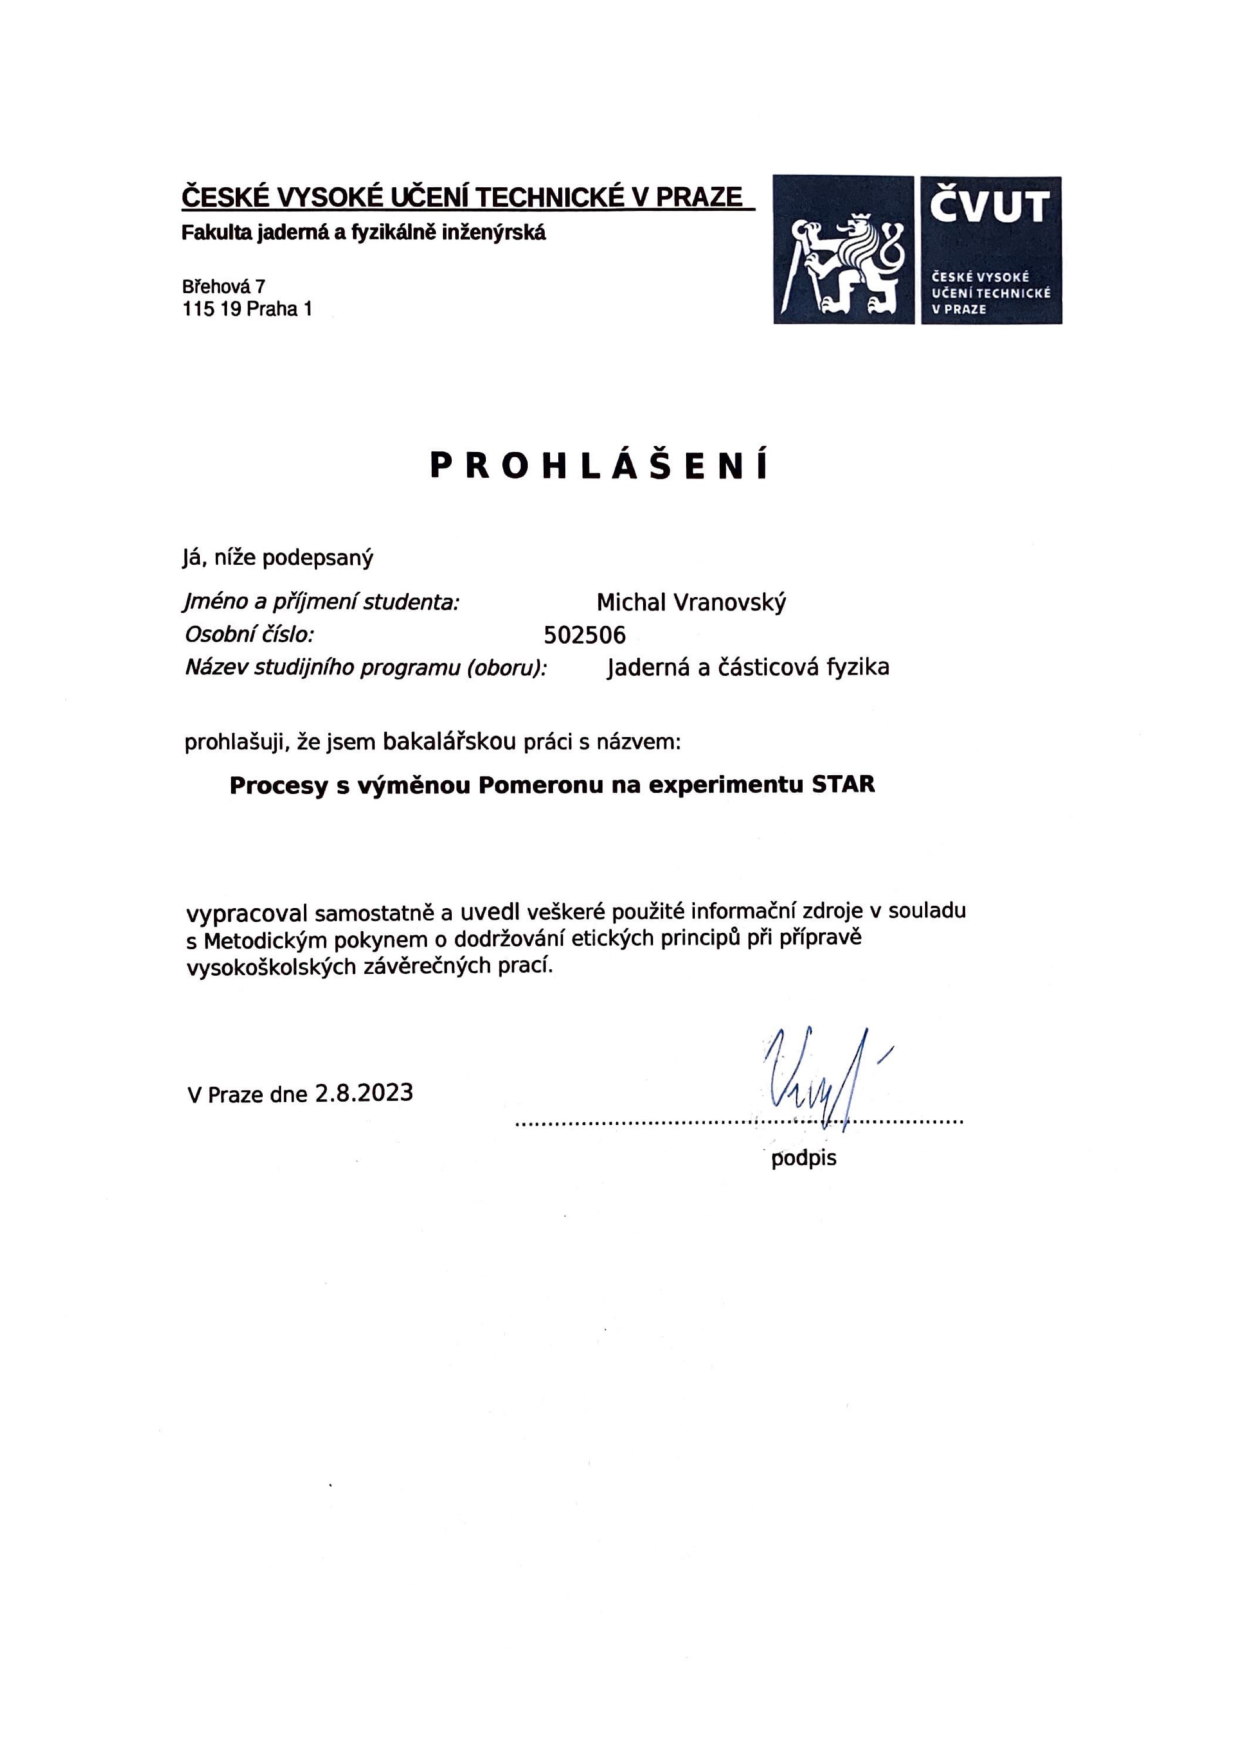
\includepdf[pages={1}]{figures/prohlaseni.pdf} % NAHRAĎTE správným souborem!



%\thispagestyle{empty}  

%~ 
%\vfill % prázdné místo. SEM NESAHEJTE!

%\noindent \tb{Prohlášení} 

%\vspace{1em} % vertikální mezera. SEM NESAHEJTE!
%\prohlaseni

%\vspace{2em}  
%\hspace{-0.5em}\begin{tabularx}{\textwidth}{X c}  
%V~\kde\ dne .................... &........................................ \\   
%    & \autor
%\end{tabularx}  

%\newpage 
%\thispagestyle{empty} 
%\

%%%%%%%%%%%% Poděkování  %%%%%%%%%%%%
\newpage
\thispagestyle{empty}

~
\vfill % prázdné místo

\noindent \tb{Acknowledgments}

\vspace{1em} % vertikální mezera
\podekovani
\begin{flushright}
\autor
\end{flushright}  % <------- tady končí stránka s poděkováním

\newpage 
\thispagestyle{empty} 
\


%%%%%%%%%%%% ABSTRAKT  %%%%%%%%%%%% 
\newpage   
\thispagestyle{empty}   

% příprava:    (na následujících 8 řádků NESAHEJTE!)
\newbox\odstavecbox
\newlength\vyskaodstavce
\newcommand\odstavec[2]{%
    \setbox\odstavecbox=\hbox{%
         \parbox[t]{#1}{#2\vrule width 0pt depth 4pt}}%
    \global\vyskaodstavce=\dp\odstavecbox
    \box\odstavecbox}
\newcommand{\delka}{118mm -2\tabcolsep} % šířka textů ve~2. sloupci tabulky

\hspace*{-0.33cm}
\begin{tabular}{p{3.1cm} l}
   {\em Název práce:} & \odstavec{\delka}{\bf\nazevcz} \\[1em]
  {\em Autor:} & \autor \\[1em]
  {\em Studijní program:} & \obor \\[1em]
  
  %{\em Obor:} & \obor \\
  {\em Druh práce:} & \druh \\[1em]
  {\em Vedoucí práce:} & \odstavec{\delka}{\vedouci,  \pracovisteVed} \\
  {\em Konzultant:} & \odstavec{\delka}{\konzultant,  \pracovisteKonz}\\ [1em] 
\end{tabular}  

{\em Abstrakt:} ~ \abstrCZ   \\[1em]
\hspace*{-0.33cm}
\begin{tabular}{p{3.1cm} l}
  {\em Klíčové slova:} & \odstavec{\delka}{\klicova} \\[1em]
\end{tabular} 

\hspace*{-0.33cm}
\begin{tabular}{p{3.1cm} l}
  {\em Title:} & \odstavec{\delka}{\bf \nazeven} \\[1em]  
  
  {\em Author:} & \autor \\[1em]
\end{tabular}  
{\em Abstract:} ~ \abstrEN   \\[1em]
\hspace*{-0.33cm}
\begin{tabular}{p{3.1cm} l}
  {\em Key words:} & \odstavec{\delka}{\keyword} 
\end{tabular}